\chapter*{Introduction}
\kaitodo[inline]{read chapter/section}
% ##################################################################################################################

\begin{center} 
\includegraphics[width=0.3\textwidth, angle=0]{frontmatter/figures/MATSimBook} \end{center}

% ##################################################################################################################
%The intense \gls{matsim} development and research during the last few years has generated an extensive body of knowledge with numerous studies, dissertations and projects in research and practice. It is time to put together all the floating pieces and contextualize them in a consistent and coherent manner, as illustrated by the figure above. 
%
%There have been many authors and three editors contributing to this book. Authors come from the \gls{matsim} team but also from the wider community. Chapters have been written by the respective software contributor or researcher whenever possible, which ensures capturing the most complete and detailed knowledge.
%
The book is intended to give the new \gls{matsim} user a quick start in running \gls{matsim} and also provide the more experienced \gls{matsim} user and the \gls{matsim} developer with details on how to extend \gls{matsim} by plugging in available modules (\ie the \glspl{contribution}) and by programming against the \gls{matsim} \gls{api} to implement their own \gls{matsim} \glspl{extension}. One of this book's most important goals is to contextualize the methods used in \gls{matsim} in a broader theoretical background. By compiling our conceptual insights on \gls{matsim} gained over the years, the book also contributes to methodological discussion on joint \gls{microsimulation} of travel demand and traffic flow, a relatively new field, or---more generally---spatial demand and its congestion generation.

The book is divided into four parts, focused on \emph{using}, \emph{extending} and \emph{understanding} \gls{matsim}, as well as providing practical, technical and methodological information. The last part presents an impressive array of  \gls{matsim} scenarios that have now been created around the world. %\ah{beschreiben, wie man nach und nach inhaltlich tiefer geht. Verwobenheit des Buches ansprechen.}

\clearpage
% -----------------
\begin{wrapfigure}[6]{r}{0.17\textwidth}
\vspace{-5pt}
  \begin{center}
    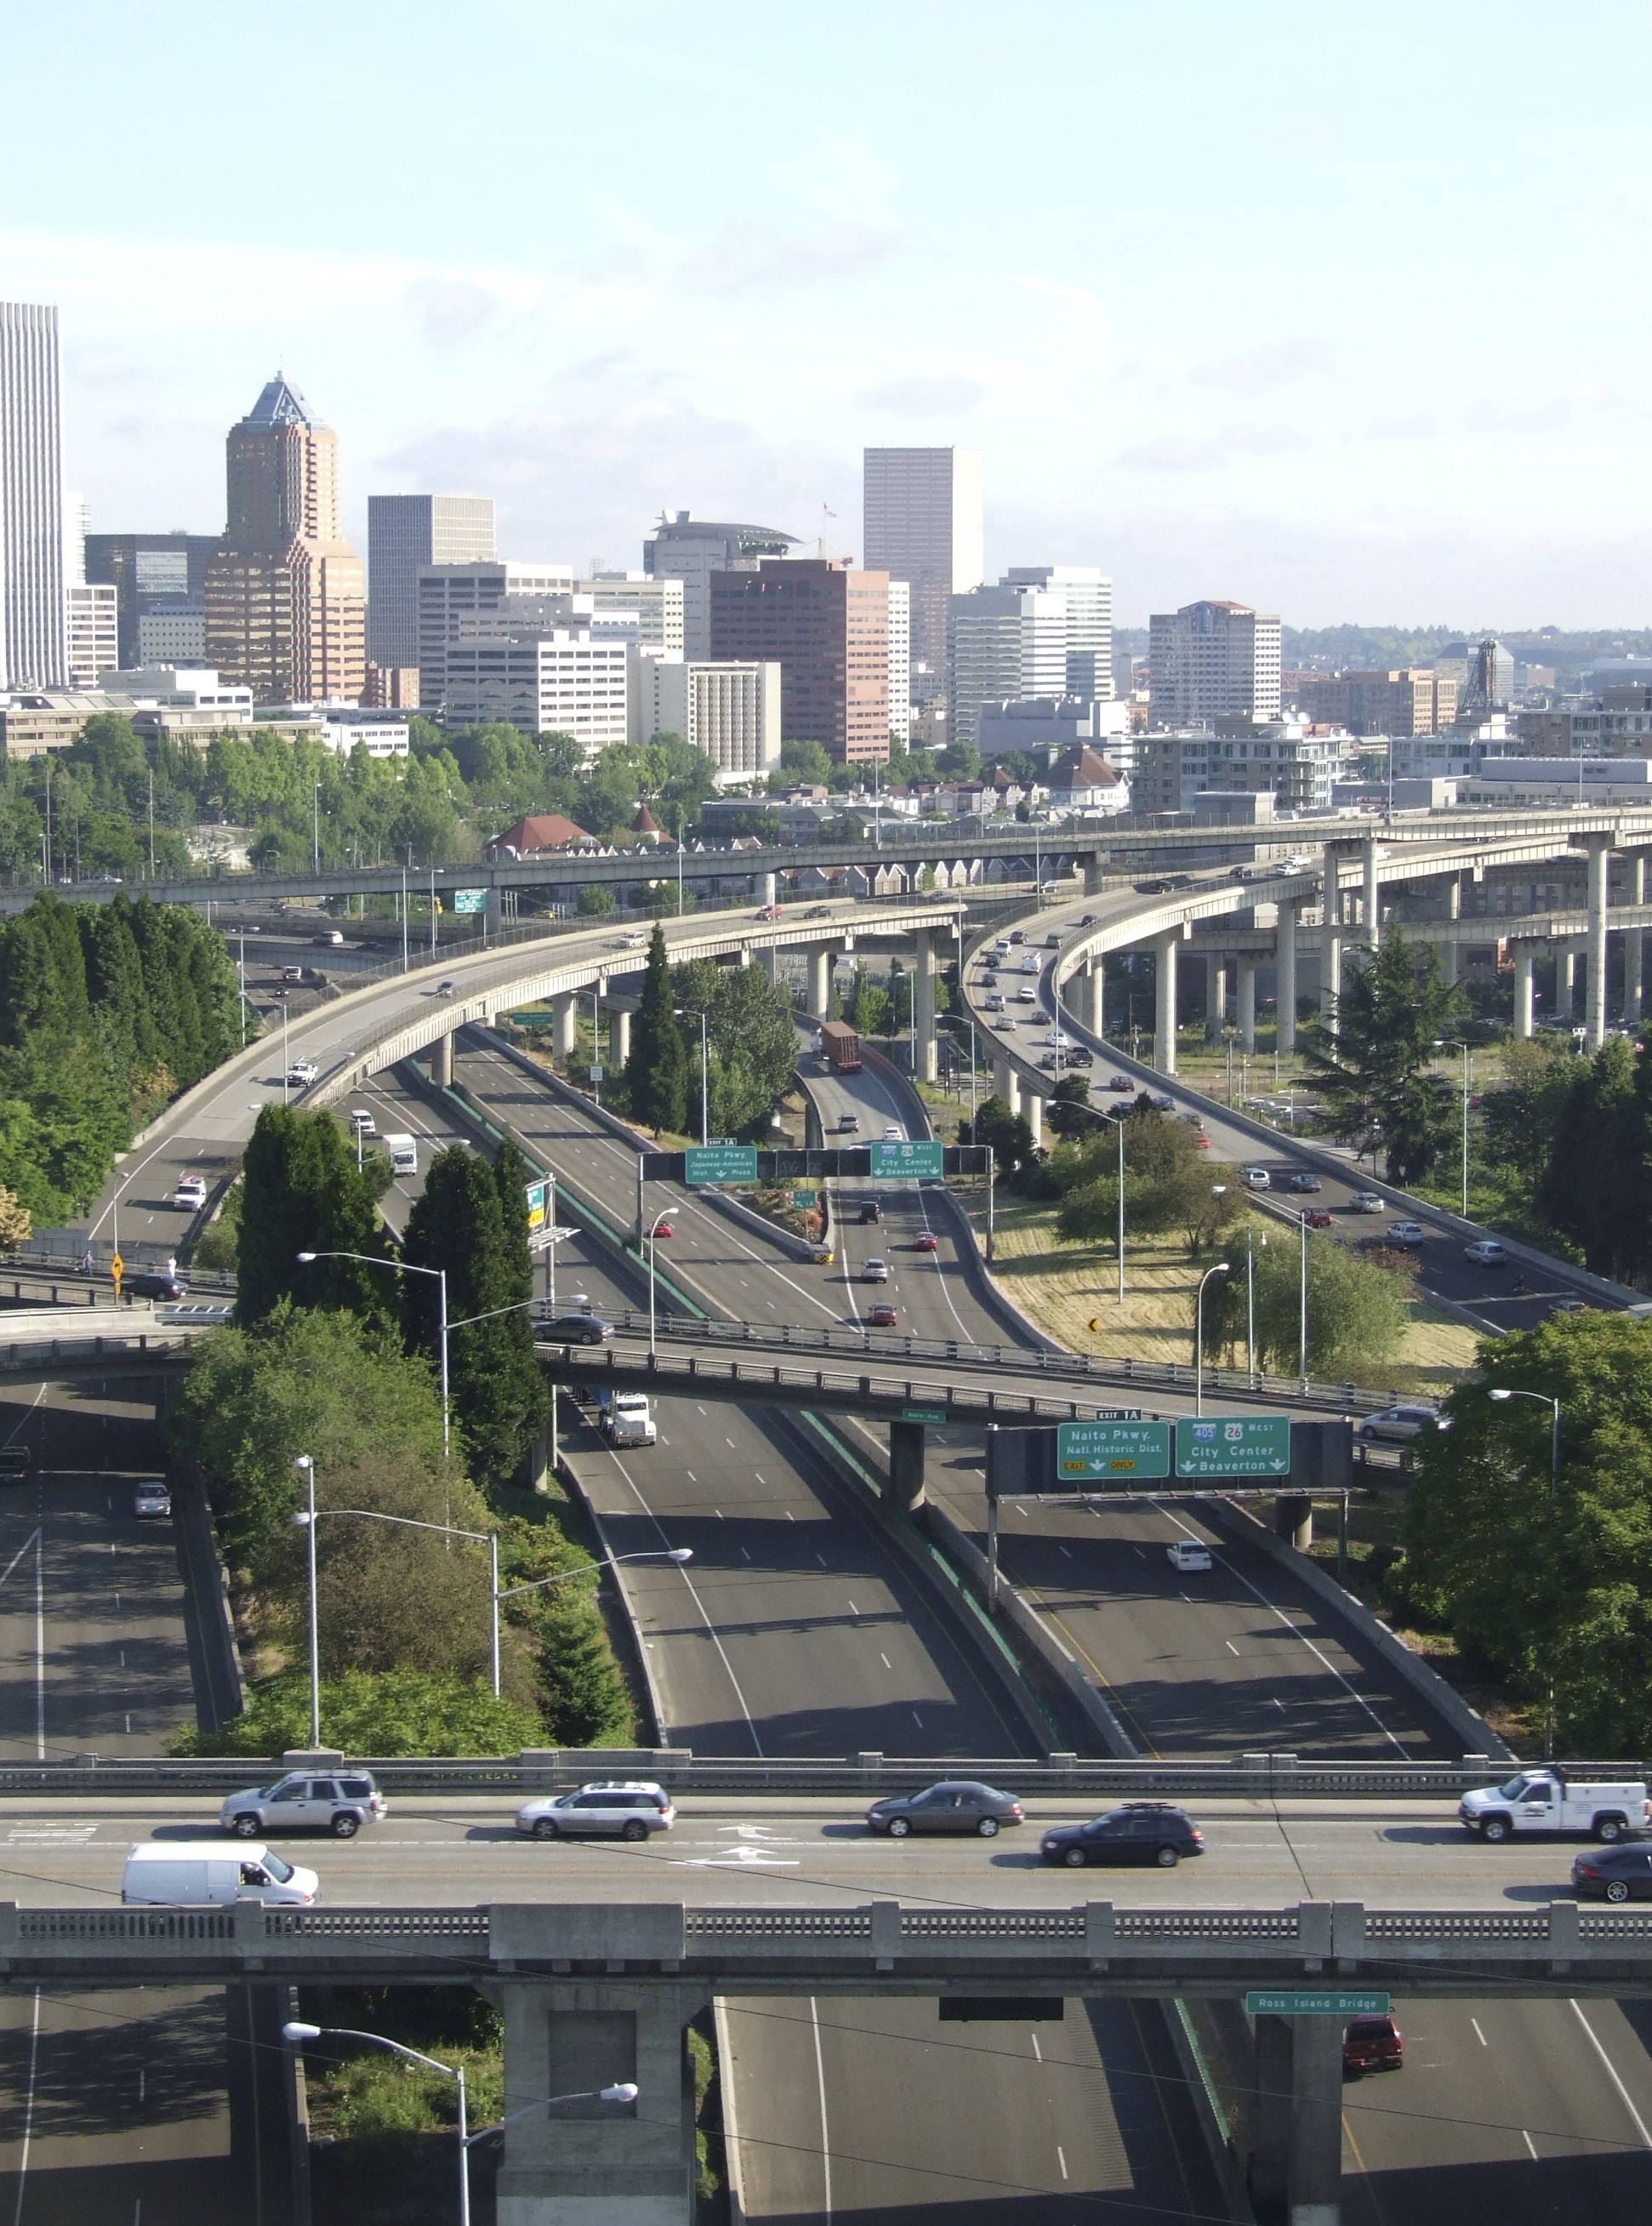
\includegraphics[width=0.15\textwidth]{images/DSCF2906.jpg}
  \end{center}
\end{wrapfigure}
\textbf{Part I: Using \acrshort{matsim}}\\
This part enables users to run \gls{matsim} with only the \gls{configfile}, a population and a network. They are given general information to assess whether \gls{matsim} is a suitable tool and method for their specific research question.

Chapter~\ref{ch:introducing} introduces the \gls{matsim} basics, including its traffic flow model and underlying co-evolutionary principle. 
Chapter~\ref{ch:lgstarted} shows the \gls{matsim} novice how to set up and run a basic \gls{matsim} \gls{scenario}. 
Chapter~\ref{ch:configuring} lists the \gls{configfile}'s options available for basic scenarios containing \gls{configfile}, a population and a network.  
Scoring is central to \gls{matsim}; a full chapter, Chapter~\ref{ch:scoring}, scrutinizes scoring. 

% -----------------
\begin{wrapfigure}[6]{r}{0.17\textwidth}
\vspace{-10pt}
  \begin{center}
    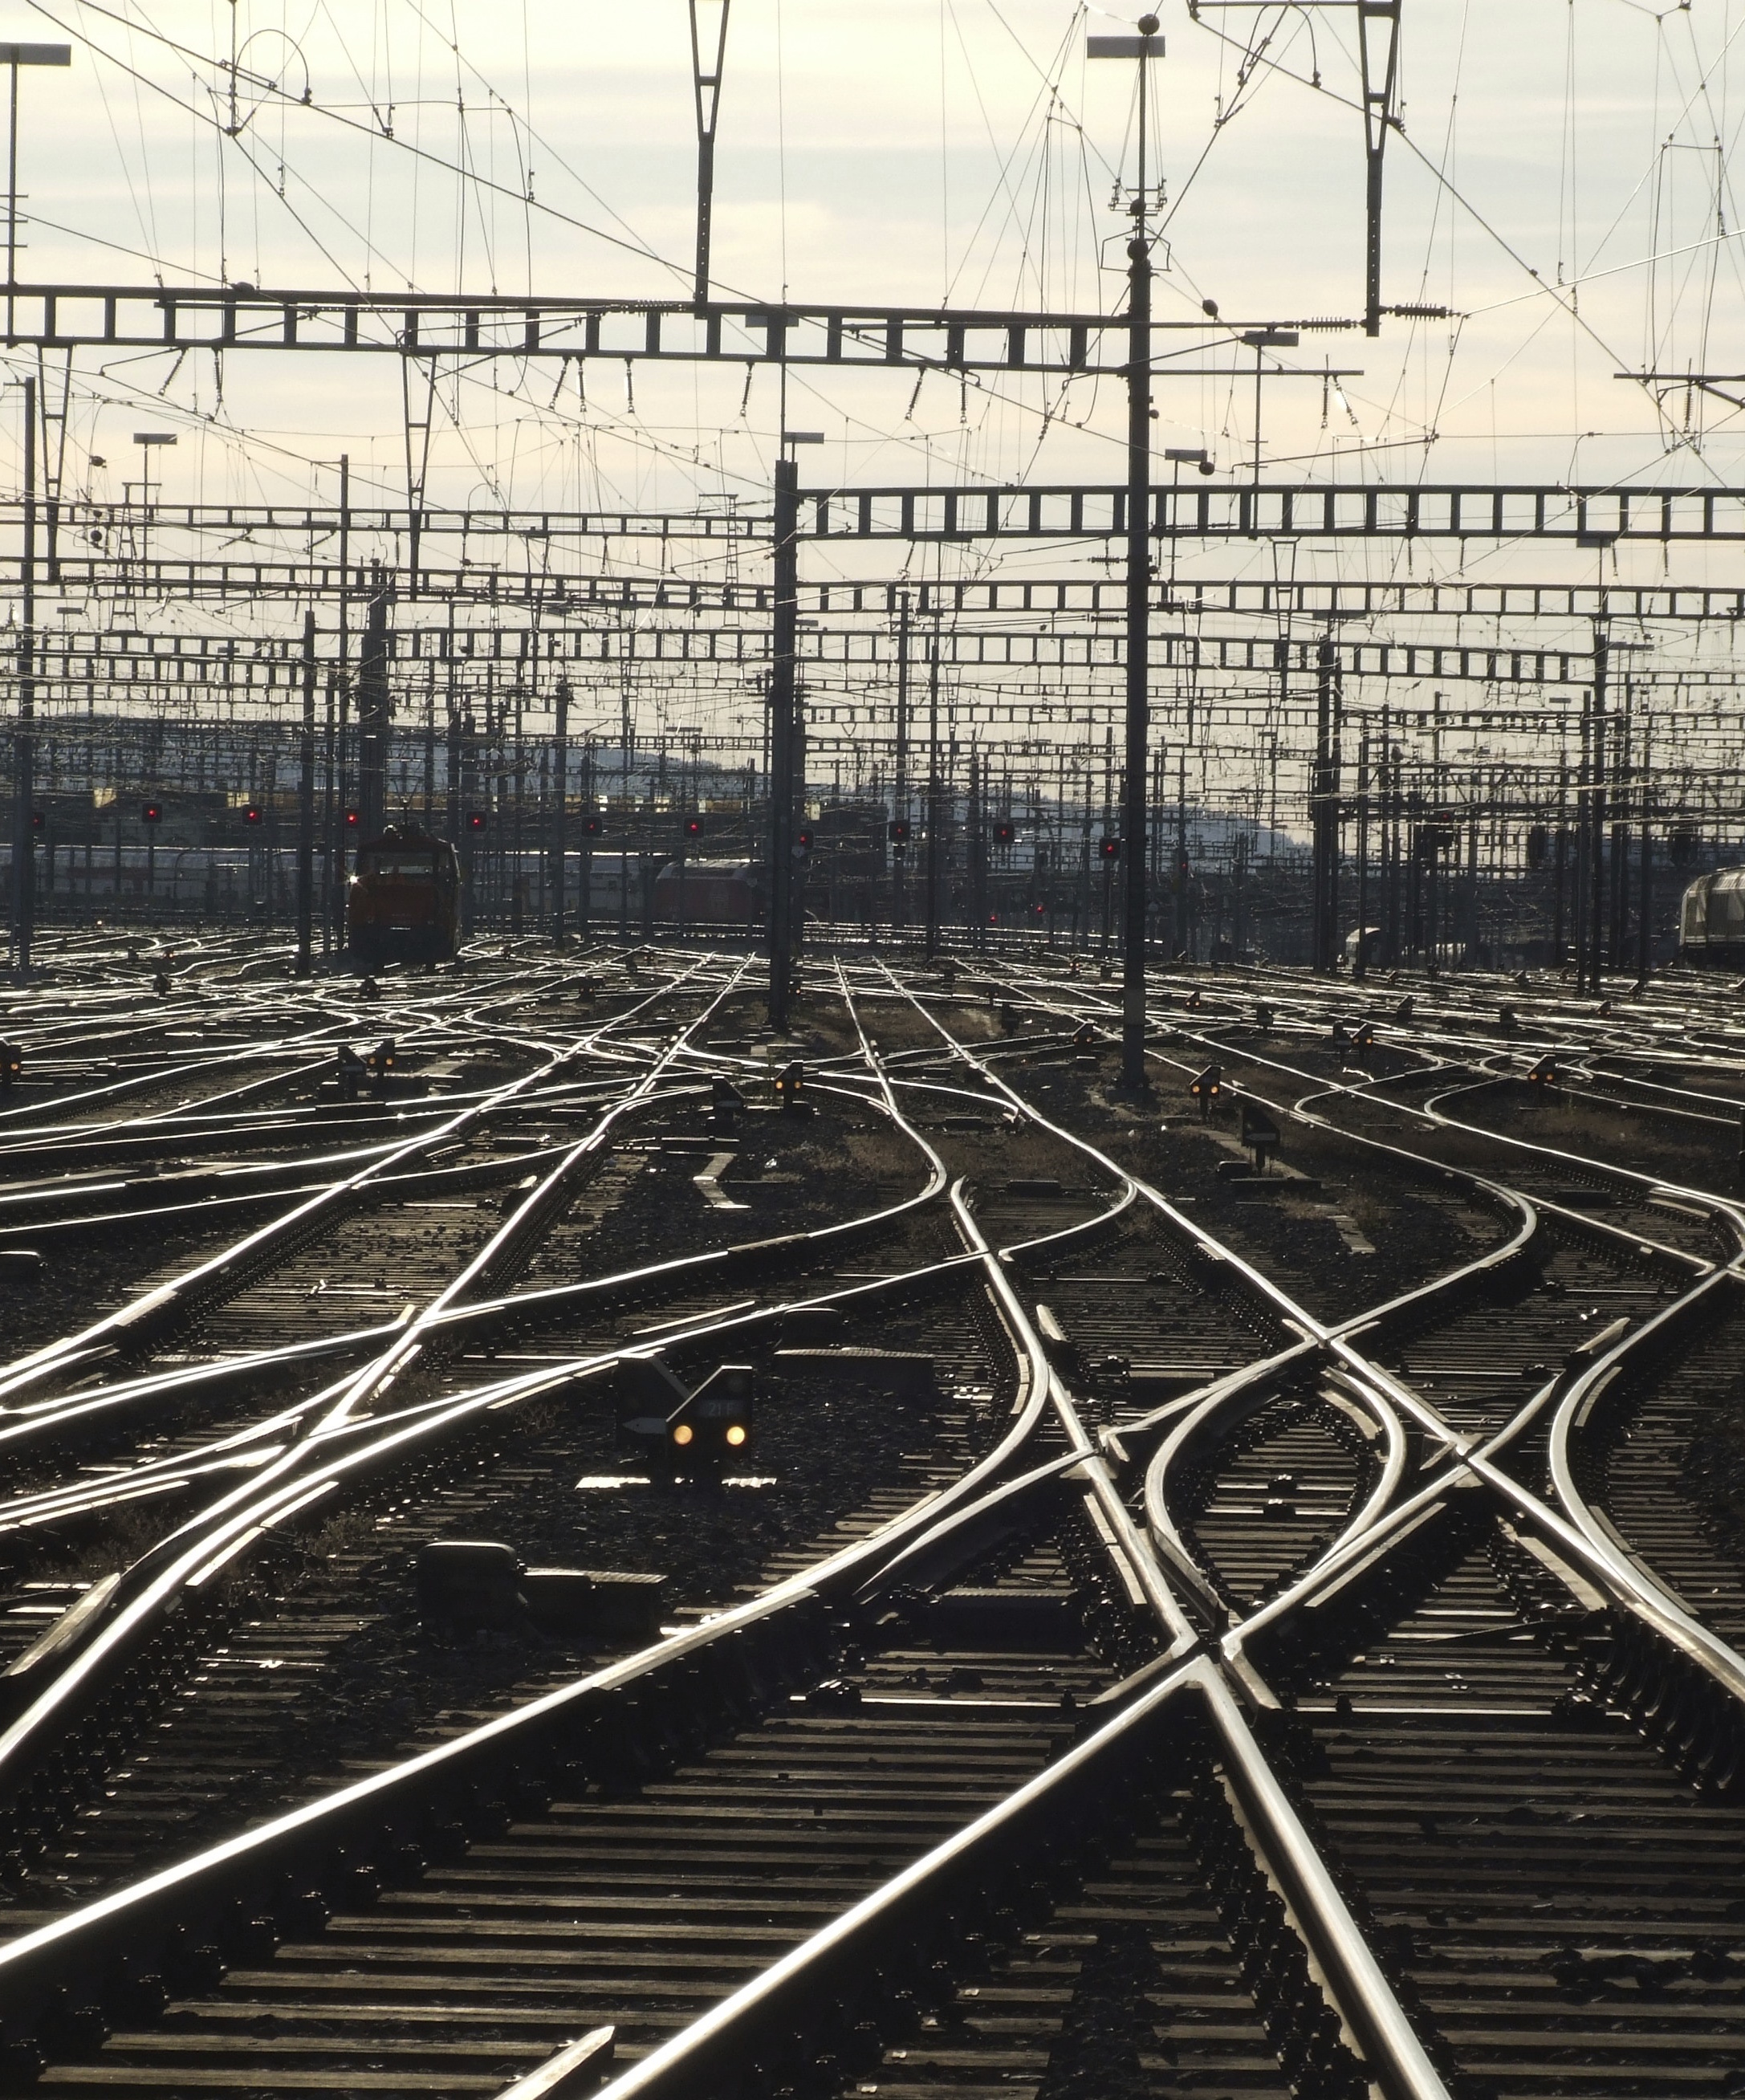
\includegraphics[width=0.15\textwidth]{images/DSCF5871.jpg}
  \end{center}
\end{wrapfigure}
\textbf{Part II: Extending \acrshort{matsim}}\\
This part presents significant technical information on how to extend the base functionality of \gls{matsim} by additional input data beyond \gls{configfile}, population and network, as well as by programming against the \gls{api}. 

Chapter~\ref{ch:modules} introduces \gls{matsim}'s modular architecture and explains how to use the available \glspl{module} introduced in Chapters~\ref{ch:destinationchoice} through \ref{ch:businessanalytics}. Chapter~\ref{ch:discontinued} describes modules that were important in the past, but whose development is discontinued.
Chapter~\ref{ch:developmentprocess} briefly describes \gls{matsim} organization, \ie its development process, code structure, the team and the community and summarizes their development tools. 
Chapter~\ref{ch:extensionpoints} goes one step further and explains to readers how to write their own \gls{matsim} \gls{extension} and how to then contribute it to \gls{matsim}, including details about points where \gls{matsim} can be extended; it also digs a bit deeper and provides details about the very central \gls{matsim} concept of \glspl{event}. Explanation about  how to add a \lstinline|Listener| and write a customized \lstinline|Controler| is also found here.

% -----------------
\begin{wrapfigure}[7]{r}{0.17\textwidth}
\vspace{-10pt}
  \begin{center}
    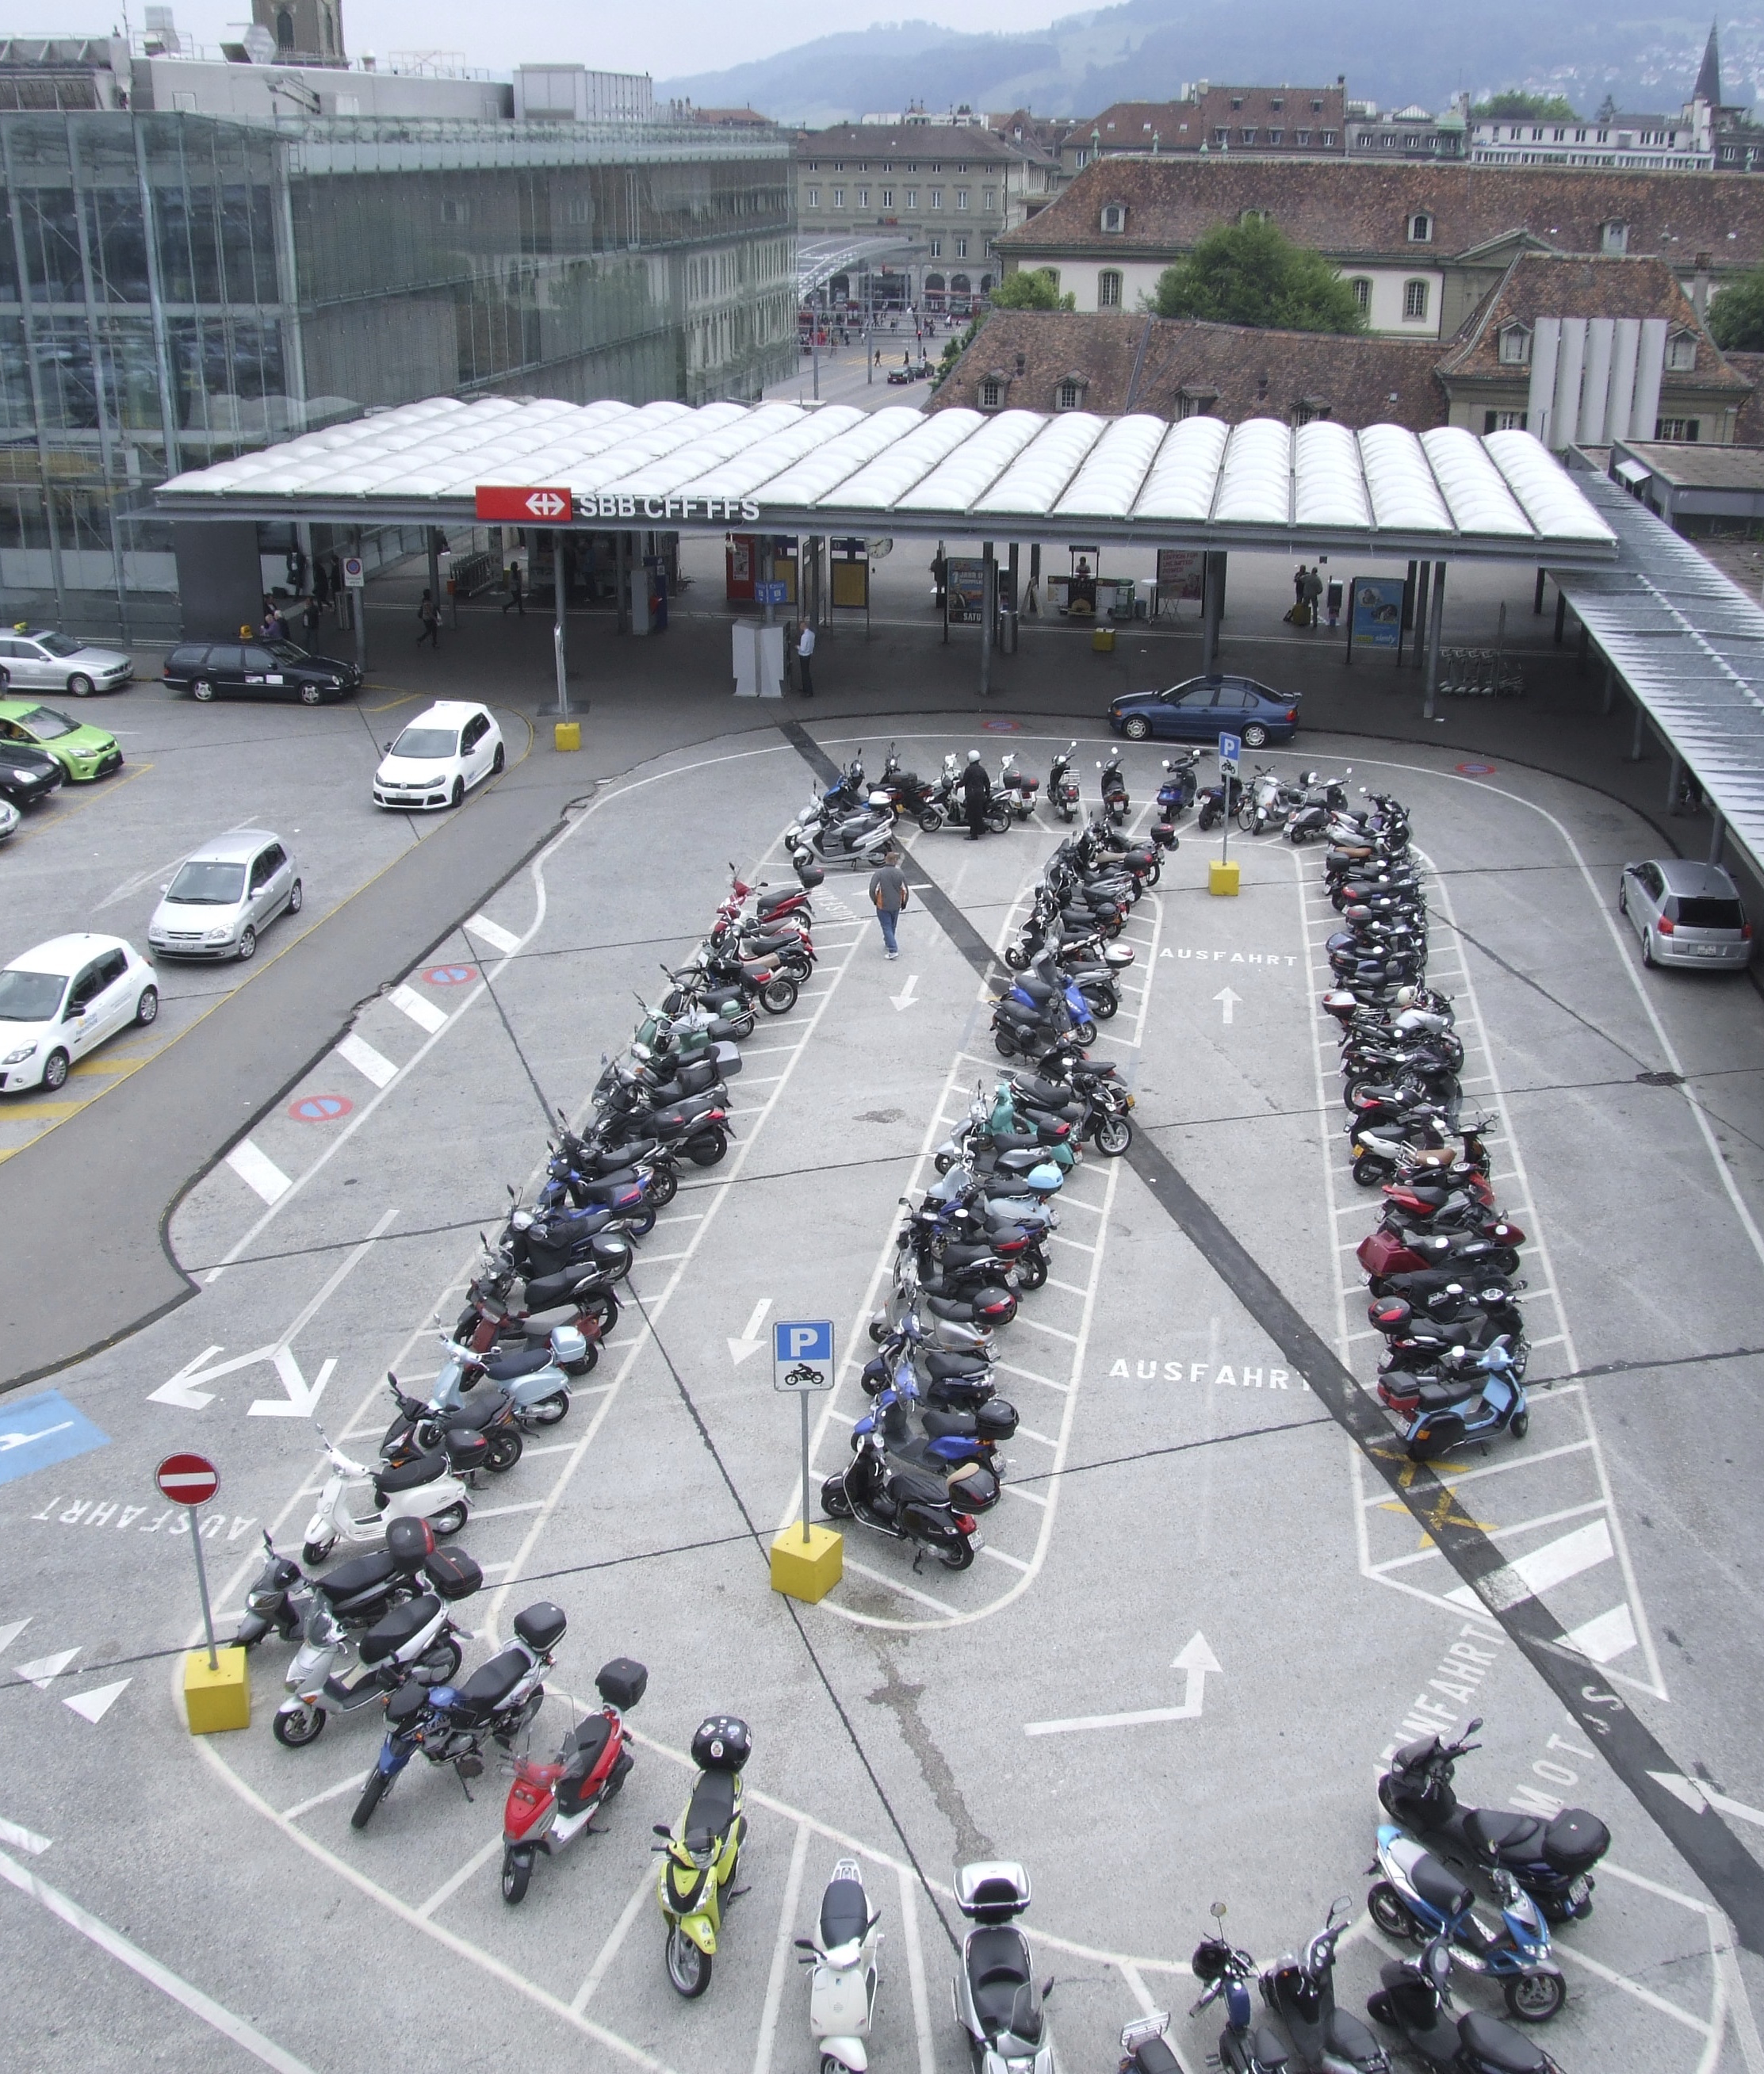
\includegraphics[width=0.15\textwidth]{images/DSCF5900.jpg}
  \end{center}
\end{wrapfigure}
\textbf{Part III: Understanding \acrshort{matsim}}\\
%\ah{Gunnar fragen, ob er hier eine gehaltvollere Zusammenfassung/Vorschau machen möchte}
%\gunnar{Von mir aus ist das hinreichend, es sei denn, jemand m\"ochte, dass ich den kommenden Abschnitt irgendwie ausbaue.}
%\ah{ok, then let us keep it like that}
%
This part presents theoretical aspects underlying the previous two sections. For example, the \gls{matsim} \gls{score} is no longer simply denoted by $S$ without interpretation, but is here contextualized within the discrete choice framework (Chapter~\ref{ch:discretechoice}) and becomes \gls{utility}, commonly denoted by $U$. 
The first chapter, Chapter~\ref{ch:history} starts with a summary of \gls{matsim}'s history, written by Kai Nagel and Kay W.\ Axhausen, \gls{matsim}'s ``fathers''. 
Chapter~\ref{ch:abta} then elaborates on agent-based traffic assignment and qualitatively contextualizes \gls{matsim} within classical concepts. Here, focus is on development from static to dynamic \gls{trafficassignment} and, finally, agent-based \gls{trafficassignment}.  
Chapter~\ref{ch:montecarlo} quantitatively contextualizes \gls{matsim} within classical concepts by presenting it as a fundamentally stochastic tool, based on random distributions and understandable as a Monte Carlo engine.
Chapter~\ref{ch:kinematicwaves} analyzes \gls{matsim}'s traffic flow model in relation to kinematic waves and Chapter~\ref{ch:economicEval} provides an economic view on \gls{matsim}. 

% -----------------
\begin{wrapfigure}[7]{r}{0.17\textwidth}
\vspace{-10pt}
  \begin{center}
    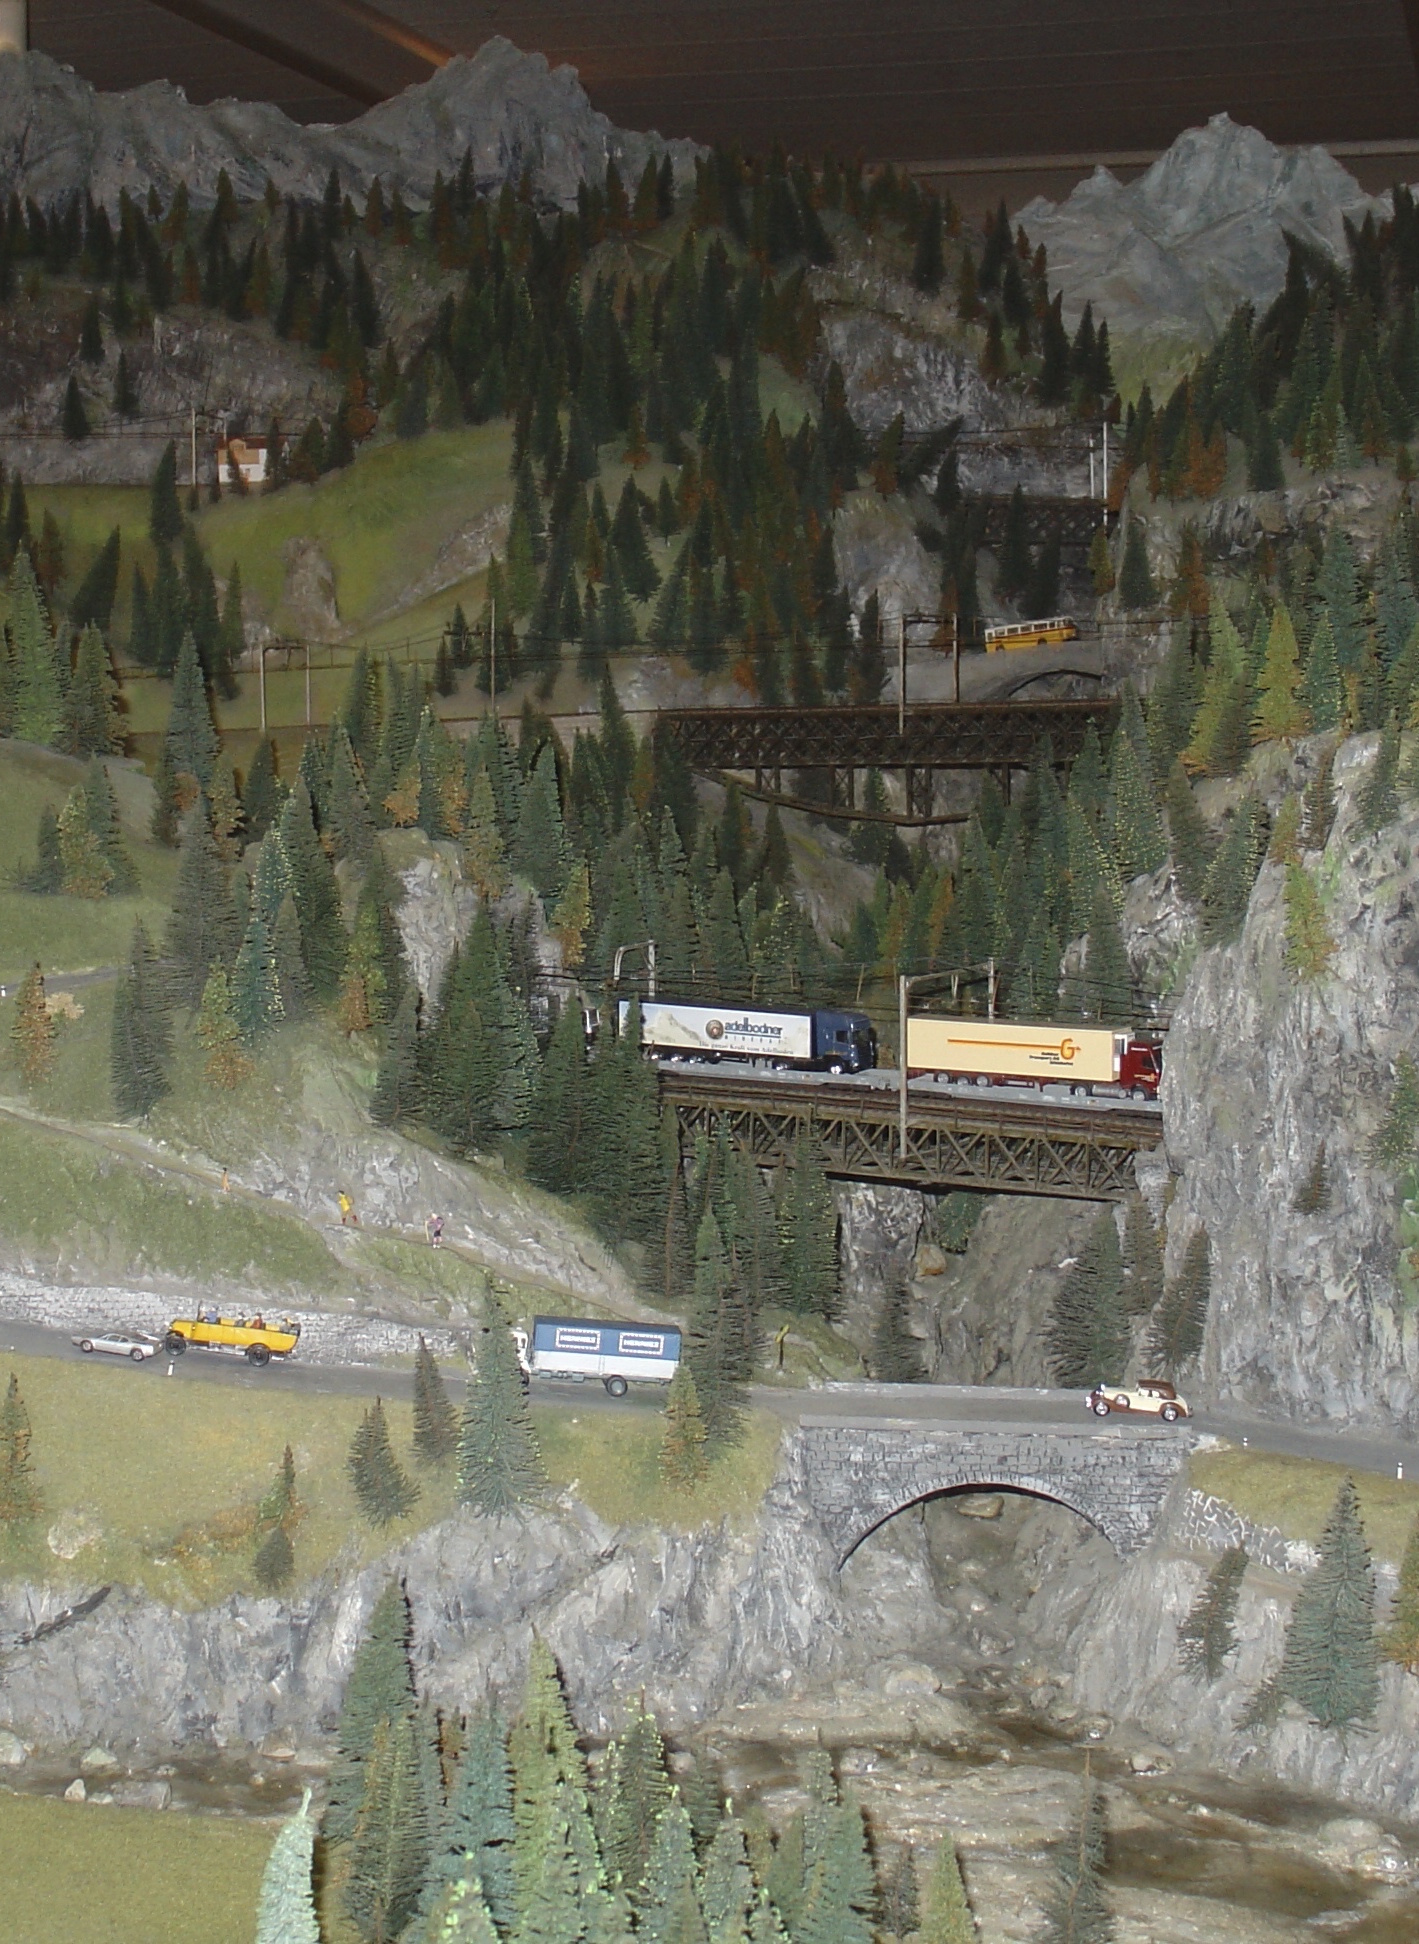
\includegraphics[width=0.15\textwidth]{images/DSC00233.jpg}
  \end{center}
\end{wrapfigure}
\textbf{Part IV: Scenarios}\\
At this point, when readers have a complete picture of \gls{matsim} and are ready to set up their own real-world \gls{matsim} \gls{scenario}, Chapters~\ref{ch:scenarios} through~\ref{ch:yarrawonga} show them the numerous and highly varied scenarios that have been implemented around the world.

% -----------------
\vskip 1cm
The book concludes with a discussion of promising research avenues (Chapter~\ref{ch:researchavenues}).

% ##################################################################################################################
\section*{Related Material}

The book concentrates on the more stable aspects of \gls{matsim} application and development.  In the future, revisions of Chapters~\ref{ch:introducing} to~\ref{ch:modules} will be presented once a year.  Additional material is referenced from \url{http://matsim.org}, for example under \url{http://matsim.org/docs}, \url{http://matsim.org/javadoc}, \url{http://matsim.org/extensions}, \url{http://matsim.org/faq}, or \url{http://matsim.org/issuetracker}.


%% , while the practical issues, such as specific configurations or code details---usually being part of manuals---can primarily be found in the \gls{matsim} user guide (shipped with the \gls{matsim} releases) and provided on the \gls{matsim} web page \citep[][]{MATSim_Userguide_2015}. \todokai{rm usrguide}

% ##################################################################################################################

% Local Variables:
% mode: latex
% mode: reftex
% mode: visual-line
% TeX-master: "../main"
% comment-padding: 1
% fill-column: 9999
% End: 
